\documentclass[1p]{elsarticle_modified}
%\bibliographystyle{elsarticle-num}

%\usepackage[colorlinks]{hyperref}
%\usepackage{abbrmath_seonhwa} %\Abb, \Ascr, \Acal ,\Abf, \Afrak
\usepackage{amsfonts}
\usepackage{amssymb}
\usepackage{amsmath}
\usepackage{amsthm}
\usepackage{scalefnt}
\usepackage{amsbsy}
\usepackage{kotex}
\usepackage{caption}
\usepackage{subfig}
\usepackage{color}
\usepackage{graphicx}
\usepackage{xcolor} %% white, black, red, green, blue, cyan, magenta, yellow
\usepackage{float}
\usepackage{setspace}
\usepackage{hyperref}

\usepackage{tikz}
\usetikzlibrary{arrows}

\usepackage{multirow}
\usepackage{array} % fixed length table
\usepackage{hhline}

%%%%%%%%%%%%%%%%%%%%%
\makeatletter
\renewcommand*\env@matrix[1][\arraystretch]{%
	\edef\arraystretch{#1}%
	\hskip -\arraycolsep
	\let\@ifnextchar\new@ifnextchar
	\array{*\c@MaxMatrixCols c}}
\makeatother %https://tex.stackexchange.com/questions/14071/how-can-i-increase-the-line-spacing-in-a-matrix
%%%%%%%%%%%%%%%

\usepackage[normalem]{ulem}

\newcommand{\msout}[1]{\ifmmode\text{\sout{\ensuremath{#1}}}\else\sout{#1}\fi}
%SOURCE: \msout is \stkout macro in https://tex.stackexchange.com/questions/20609/strikeout-in-math-mode

\newcommand{\cancel}[1]{
	\ifmmode
	{\color{red}\msout{#1}}
	\else
	{\color{red}\sout{#1}}
	\fi
}

\newcommand{\add}[1]{
	{\color{blue}\uwave{#1}}
}

\newcommand{\replace}[2]{
	\ifmmode
	{\color{red}\msout{#1}}{\color{blue}\uwave{#2}}
	\else
	{\color{red}\sout{#1}}{\color{blue}\uwave{#2}}
	\fi
}

\newcommand{\Sol}{\mathcal{S}} %segment
\newcommand{\D}{D} %diagram
\newcommand{\A}{\mathcal{A}} %arc


%%%%%%%%%%%%%%%%%%%%%%%%%%%%%5 test

\def\sl{\operatorname{\textup{SL}}(2,\Cbb)}
\def\psl{\operatorname{\textup{PSL}}(2,\Cbb)}
\def\quan{\mkern 1mu \triangleright \mkern 1mu}

\theoremstyle{definition}
\newtheorem{thm}{Theorem}[section]
\newtheorem{prop}[thm]{Proposition}
\newtheorem{lem}[thm]{Lemma}
\newtheorem{ques}[thm]{Question}
\newtheorem{cor}[thm]{Corollary}
\newtheorem{defn}[thm]{Definition}
\newtheorem{exam}[thm]{Example}
\newtheorem{rmk}[thm]{Remark}
\newtheorem{alg}[thm]{Algorithm}

\newcommand{\I}{\sqrt{-1}}
\begin{document}

%\begin{frontmatter}
%
%\title{Boundary parabolic representations of knots up to 8 crossings}
%
%%% Group authors per affiliation:
%\author{Yunhi Cho} 
%\address{Department of Mathematics, University of Seoul, Seoul, Korea}
%\ead{yhcho@uos.ac.kr}
%
%
%\author{Seonhwa Kim} %\fnref{s_kim}}
%\address{Center for Geometry and Physics, Institute for Basic Science, Pohang, 37673, Korea}
%\ead{ryeona17@ibs.re.kr}
%
%\author{Hyuk Kim}
%\address{Department of Mathematical Sciences, Seoul National University, Seoul 08826, Korea}
%\ead{hyukkim@snu.ac.kr}
%
%\author{Seokbeom Yoon}
%\address{Department of Mathematical Sciences, Seoul National University, Seoul, 08826,  Korea}
%\ead{sbyoon15@snu.ac.kr}
%
%\begin{abstract}
%We find all boundary parabolic representation of knots up to 8 crossings.
%
%\end{abstract}
%\begin{keyword}
%    \MSC[2010] 57M25 
%\end{keyword}
%
%\end{frontmatter}

%\linenumbers
%\tableofcontents
%
\newcommand\colored[1]{\textcolor{white}{\rule[-0.35ex]{0.8em}{1.4ex}}\kern-0.8em\color{red} #1}%
%\newcommand\colored[1]{\textcolor{white}{ #1}\kern-2.17ex	\textcolor{white}{ #1}\kern-1.81ex	\textcolor{white}{ #1}\kern-2.15ex\color{red}#1	}

{\Large $\underline{12n_{0865}~(K12n_{0865})}$}

\setlength{\tabcolsep}{10pt}
\renewcommand{\arraystretch}{1.6}
\vspace{1cm}\begin{tabular}{m{100pt}>{\centering\arraybackslash}m{274pt}}
\multirow{5}{120pt}{
	\centering
	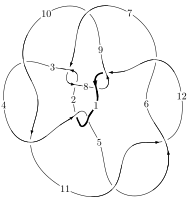
\includegraphics[width=112pt]{../../../GIT/diagram.site/Diagrams/png/2954_12n_0865.png}\\
\ \ \ A knot diagram\footnotemark}&
\allowdisplaybreaks
\textbf{Linearized knot diagam} \\
\cline{2-2}
 &
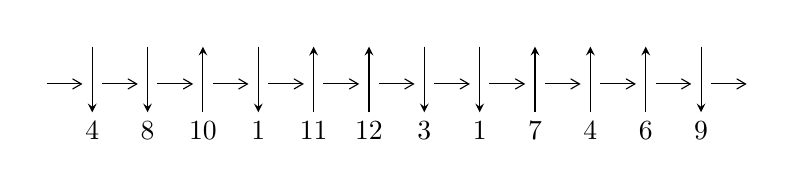
\begin{tikzpicture}[x=20pt, y=17pt]
	% nodes
	\node (C0) at (0, 0) {};
	\node (C1) at (1, 0) {};
	\node (C1U) at (1, +1) {};
	\node (C1D) at (1, -1) {4};

	\node (C2) at (2, 0) {};
	\node (C2U) at (2, +1) {};
	\node (C2D) at (2, -1) {8};

	\node (C3) at (3, 0) {};
	\node (C3U) at (3, +1) {};
	\node (C3D) at (3, -1) {10};

	\node (C4) at (4, 0) {};
	\node (C4U) at (4, +1) {};
	\node (C4D) at (4, -1) {1};

	\node (C5) at (5, 0) {};
	\node (C5U) at (5, +1) {};
	\node (C5D) at (5, -1) {11};

	\node (C6) at (6, 0) {};
	\node (C6U) at (6, +1) {};
	\node (C6D) at (6, -1) {12};

	\node (C7) at (7, 0) {};
	\node (C7U) at (7, +1) {};
	\node (C7D) at (7, -1) {3};

	\node (C8) at (8, 0) {};
	\node (C8U) at (8, +1) {};
	\node (C8D) at (8, -1) {1};

	\node (C9) at (9, 0) {};
	\node (C9U) at (9, +1) {};
	\node (C9D) at (9, -1) {7};

	\node (C10) at (10, 0) {};
	\node (C10U) at (10, +1) {};
	\node (C10D) at (10, -1) {4};

	\node (C11) at (11, 0) {};
	\node (C11U) at (11, +1) {};
	\node (C11D) at (11, -1) {6};

	\node (C12) at (12, 0) {};
	\node (C12U) at (12, +1) {};
	\node (C12D) at (12, -1) {9};
	\node (C13) at (13, 0) {};

	% arrows
	\draw[->,>={angle 60}]
	(C0) edge (C1) (C1) edge (C2) (C2) edge (C3) (C3) edge (C4) (C4) edge (C5) (C5) edge (C6) (C6) edge (C7) (C7) edge (C8) (C8) edge (C9) (C9) edge (C10) (C10) edge (C11) (C11) edge (C12) (C12) edge (C13) ;	\draw[->,>=stealth]
	(C1U) edge (C1D) (C2U) edge (C2D) (C3D) edge (C3U) (C4U) edge (C4D) (C5D) edge (C5U) (C6D) edge (C6U) (C7U) edge (C7D) (C8U) edge (C8D) (C9D) edge (C9U) (C10D) edge (C10U) (C11D) edge (C11U) (C12U) edge (C12D) ;
	\end{tikzpicture} \\
\hhline{~~} \\& 
\textbf{Solving Sequence} \\ \cline{2-2} 
 &
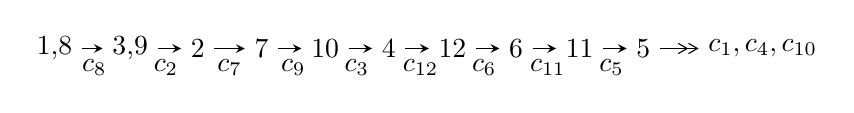
\begin{tikzpicture}[x=23pt, y=7pt]
	% node
	\node (A0) at (-1/8, 0) {1,8};
	\node (A1) at (17/16, 0) {3,9};
	\node (A2) at (17/8, 0) {2};
	\node (A3) at (25/8, 0) {7};
	\node (A4) at (33/8, 0) {10};
	\node (A5) at (41/8, 0) {4};
	\node (A6) at (49/8, 0) {12};
	\node (A7) at (57/8, 0) {6};
	\node (A8) at (65/8, 0) {11};
	\node (A9) at (73/8, 0) {5};
	\node (C1) at (1/2, -1) {$c_{8}$};
	\node (C2) at (13/8, -1) {$c_{2}$};
	\node (C3) at (21/8, -1) {$c_{7}$};
	\node (C4) at (29/8, -1) {$c_{9}$};
	\node (C5) at (37/8, -1) {$c_{3}$};
	\node (C6) at (45/8, -1) {$c_{12}$};
	\node (C7) at (53/8, -1) {$c_{6}$};
	\node (C8) at (61/8, -1) {$c_{11}$};
	\node (C9) at (69/8, -1) {$c_{5}$};
	\node (A10) at (11, 0) {$c_{1},c_{4},c_{10}$};

	% edge
	\draw[->,>=stealth]	
	(A0) edge (A1) (A1) edge (A2) (A2) edge (A3) (A3) edge (A4) (A4) edge (A5) (A5) edge (A6) (A6) edge (A7) (A7) edge (A8) (A8) edge (A9) ;
	\draw[->>,>={angle 60}]	
	(A9) edge (A10);
\end{tikzpicture} \\ 

\end{tabular} \\

\footnotetext{
The image of knot diagram is generated by the software ``\textbf{Draw programme}" developed by Andrew Bartholomew(\url{http://www.layer8.co.uk/maths/draw/index.htm\#Running-draw}), where we modified some parts for our purpose(\url{https://github.com/CATsTAILs/LinksPainter}).
}\phantom \\ \newline 
\centering \textbf{Ideals for irreducible components\footnotemark of $X_{\text{par}}$} 
 
\begin{align*}
I^u_{1}&=\langle 
5.21913\times10^{261} u^{74}-9.56885\times10^{261} u^{73}+\cdots+2.67203\times10^{264} b+1.08376\times10^{265},\\
\phantom{I^u_{1}}&\phantom{= \langle  }-1.00658\times10^{265} u^{74}+2.74878\times10^{266} u^{73}+\cdots+6.32123\times10^{268} a-6.89423\times10^{270},\\
\phantom{I^u_{1}}&\phantom{= \langle  }u^{75}-2 u^{74}+\cdots-55407 u-23657\rangle \\
I^u_{2}&=\langle 
2.91037\times10^{16} u^{25}+4.54222\times10^{16} u^{24}+\cdots+3.82887\times10^{16} b+3.01035\times10^{16},\\
\phantom{I^u_{2}}&\phantom{= \langle  }4.61911\times10^{16} u^{25}+3.17301\times10^{16} u^{24}+\cdots+3.82887\times10^{16} a+1.83622\times10^{17},\;u^{26}+u^{25}+\cdots+2 u-1\rangle \\
\\
\end{align*}
\raggedright * 2 irreducible components of $\dim_{\mathbb{C}}=0$, with total 101 representations.\\
\footnotetext{All coefficients of polynomials are rational numbers. But the coefficients are sometimes approximated in decimal forms when there is not enough margin.}
\newpage
\renewcommand{\arraystretch}{1}
\centering \section*{I. $I^u_{1}= \langle 5.22\times10^{261} u^{74}-9.57\times10^{261} u^{73}+\cdots+2.67\times10^{264} b+1.08\times10^{265},\;-1.01\times10^{265} u^{74}+2.75\times10^{266} u^{73}+\cdots+6.32\times10^{268} a-6.89\times10^{270},\;u^{75}-2 u^{74}+\cdots-55407 u-23657 \rangle$}
\flushleft \textbf{(i) Arc colorings}\\
\begin{tabular}{m{7pt} m{180pt} m{7pt} m{180pt} }
\flushright $a_{1}=$&$\begin{pmatrix}0\\u\end{pmatrix}$ \\
\flushright $a_{8}=$&$\begin{pmatrix}1\\0\end{pmatrix}$ \\
\flushright $a_{3}=$&$\begin{pmatrix}0.000159238 u^{74}-0.00434850 u^{73}+\cdots+263.739 u+109.065\\-0.00195324 u^{74}+0.00358111 u^{73}+\cdots+5.27007 u-4.05594\end{pmatrix}$ \\
\flushright $a_{9}=$&$\begin{pmatrix}1\\u^2\end{pmatrix}$ \\
\flushright $a_{2}=$&$\begin{pmatrix}-0.00179400 u^{74}-0.000767386 u^{73}+\cdots+269.009 u+105.009\\-0.00195324 u^{74}+0.00358111 u^{73}+\cdots+5.27007 u-4.05594\end{pmatrix}$ \\
\flushright $a_{7}=$&$\begin{pmatrix}-0.000680792 u^{74}-0.00431212 u^{73}+\cdots+427.714 u+166.774\\-0.00413535 u^{74}+0.00928373 u^{73}+\cdots-54.5059 u-43.0394\end{pmatrix}$ \\
\flushright $a_{10}=$&$\begin{pmatrix}0.000787410 u^{74}+0.00462093 u^{73}+\cdots-432.170 u-181.460\\0.00222760 u^{74}-0.00102269 u^{73}+\cdots-245.378 u-100.388\end{pmatrix}$ \\
\flushright $a_{4}=$&$\begin{pmatrix}0.00134340 u^{74}-0.00259924 u^{73}+\cdots-135.966 u-59.0588\\0.00268652 u^{74}-0.00468443 u^{73}+\cdots-198.293 u-54.9937\end{pmatrix}$ \\
\flushright $a_{12}=$&$\begin{pmatrix}u\\u^3+u\end{pmatrix}$ \\
\flushright $a_{6}=$&$\begin{pmatrix}-0.00484735 u^{74}+0.00544928 u^{73}+\cdots+371.990 u+115.623\\-0.00332545 u^{74}+0.00836454 u^{73}+\cdots-129.661 u-60.4015\end{pmatrix}$ \\
\flushright $a_{11}=$&$\begin{pmatrix}-0.0000623277 u^{74}+0.000890244 u^{73}+\cdots-13.0980 u-12.5219\\-0.00713482 u^{74}+0.0130749 u^{73}+\cdots+224.237 u+0.410665\end{pmatrix}$ \\
\flushright $a_{5}=$&$\begin{pmatrix}-0.00134340 u^{74}+0.00259924 u^{73}+\cdots+135.966 u+59.0588\\-0.00115084 u^{74}+0.0000836745 u^{73}+\cdots+161.660 u+52.9222\end{pmatrix}$\\&\end{tabular}
\flushleft \textbf{(ii) Obstruction class $= -1$}\\~\\
\flushleft \textbf{(iii) Cusp Shapes $= 0.0123355 u^{74}-0.0295724 u^{73}+\cdots+5.38788 u+130.186$}\\~\\
\newpage\renewcommand{\arraystretch}{1}
\flushleft \textbf{(iv) u-Polynomials at the component}\newline \\
\begin{tabular}{m{50pt}|m{274pt}}
Crossings & \hspace{64pt}u-Polynomials at each crossing \\
\hline $$\begin{aligned}c_{1},c_{4}\end{aligned}$$&$\begin{aligned}
&u^{75}-5 u^{74}+\cdots-5 u-1
\end{aligned}$\\
\hline $$\begin{aligned}c_{2},c_{7}\end{aligned}$$&$\begin{aligned}
&u^{75}- u^{74}+\cdots-8219 u+2154
\end{aligned}$\\
\hline $$\begin{aligned}c_{3},c_{10}\end{aligned}$$&$\begin{aligned}
&u^{75}- u^{74}+\cdots+7742 u+871
\end{aligned}$\\
\hline $$\begin{aligned}c_{5},c_{6},c_{11}\end{aligned}$$&$\begin{aligned}
&u^{75}+u^{74}+\cdots-261 u-38
\end{aligned}$\\
\hline $$\begin{aligned}c_{8},c_{12}\end{aligned}$$&$\begin{aligned}
&u^{75}+2 u^{74}+\cdots-55407 u+23657
\end{aligned}$\\
\hline $$\begin{aligned}c_{9}\end{aligned}$$&$\begin{aligned}
&u^{75}-32 u^{73}+\cdots+255320 u+43933
\end{aligned}$\\
\hline
\end{tabular}\\~\\
\newpage\renewcommand{\arraystretch}{1}
\flushleft \textbf{(v) Riley Polynomials at the component}\newline \\
\begin{tabular}{m{50pt}|m{274pt}}
Crossings & \hspace{64pt}Riley Polynomials at each crossing \\
\hline $$\begin{aligned}c_{1},c_{4}\end{aligned}$$&$\begin{aligned}
&y^{75}-41 y^{74}+\cdots-1603 y-1
\end{aligned}$\\
\hline $$\begin{aligned}c_{2},c_{7}\end{aligned}$$&$\begin{aligned}
&y^{75}+43 y^{74}+\cdots-85114943 y-4639716
\end{aligned}$\\
\hline $$\begin{aligned}c_{3},c_{10}\end{aligned}$$&$\begin{aligned}
&y^{75}-41 y^{74}+\cdots+127801658 y-758641
\end{aligned}$\\
\hline $$\begin{aligned}c_{5},c_{6},c_{11}\end{aligned}$$&$\begin{aligned}
&y^{75}-75 y^{74}+\cdots-54087 y-1444
\end{aligned}$\\
\hline $$\begin{aligned}c_{8},c_{12}\end{aligned}$$&$\begin{aligned}
&y^{75}+46 y^{74}+\cdots-10823394625 y-559653649
\end{aligned}$\\
\hline $$\begin{aligned}c_{9}\end{aligned}$$&$\begin{aligned}
&y^{75}-64 y^{74}+\cdots+57837081376 y-1930108489
\end{aligned}$\\
\hline
\end{tabular}\\~\\
\newpage\flushleft \textbf{(vi) Complex Volumes and Cusp Shapes}
$$\begin{array}{c|c|c}  
\text{Solutions to }I^u_{1}& \I (\text{vol} + \sqrt{-1}CS) & \text{Cusp shape}\\
 \hline 
\begin{aligned}
u &= \phantom{-}0.511183 + 0.869827 I \\
a &= -0.419361 - 0.809039 I \\
b &= \phantom{-}0.420218 + 0.808317 I\end{aligned}
 & \phantom{-}13.27380 - 3.79908 I & \phantom{-0.000000 } 0 \\ \hline\begin{aligned}
u &= \phantom{-}0.511183 - 0.869827 I \\
a &= -0.419361 + 0.809039 I \\
b &= \phantom{-}0.420218 - 0.808317 I\end{aligned}
 & \phantom{-}13.27380 + 3.79908 I & \phantom{-0.000000 } 0 \\ \hline\begin{aligned}
u &= \phantom{-}0.104480 + 0.979928 I \\
a &= -0.487830 + 1.092380 I \\
b &= -0.921395 - 0.828476 I\end{aligned}
 & \phantom{-}2.88960 - 2.99924 I & \phantom{-0.000000 } 0 \\ \hline\begin{aligned}
u &= \phantom{-}0.104480 - 0.979928 I \\
a &= -0.487830 - 1.092380 I \\
b &= -0.921395 + 0.828476 I\end{aligned}
 & \phantom{-}2.88960 + 2.99924 I & \phantom{-0.000000 } 0 \\ \hline\begin{aligned}
u &= -0.719155 + 0.654606 I \\
a &= -0.916349 + 0.244548 I \\
b &= \phantom{-}0.291221 + 1.266280 I\end{aligned}
 & \phantom{-}2.19050 - 4.12293 I & \phantom{-0.000000 } 0 \\ \hline\begin{aligned}
u &= -0.719155 - 0.654606 I \\
a &= -0.916349 - 0.244548 I \\
b &= \phantom{-}0.291221 - 1.266280 I\end{aligned}
 & \phantom{-}2.19050 + 4.12293 I & \phantom{-0.000000 } 0 \\ \hline\begin{aligned}
u &= -0.951833 + 0.405463 I \\
a &= \phantom{-}0.325014 - 0.059797 I \\
b &= \phantom{-}0.61564 + 1.28372 I\end{aligned}
 & \phantom{-}0.23121 - 5.24301 I & \phantom{-0.000000 } 0 \\ \hline\begin{aligned}
u &= -0.951833 - 0.405463 I \\
a &= \phantom{-}0.325014 + 0.059797 I \\
b &= \phantom{-}0.61564 - 1.28372 I\end{aligned}
 & \phantom{-}0.23121 + 5.24301 I & \phantom{-0.000000 } 0 \\ \hline\begin{aligned}
u &= \phantom{-}0.105252 + 0.958516 I \\
a &= \phantom{-}1.006380 - 0.197424 I \\
b &= -0.965324 + 0.714891 I\end{aligned}
 & \phantom{-}2.78360 + 2.13158 I & \phantom{-}5.83242 + 0. I\phantom{ +0.000000I} \\ \hline\begin{aligned}
u &= \phantom{-}0.105252 - 0.958516 I \\
a &= \phantom{-}1.006380 + 0.197424 I \\
b &= -0.965324 - 0.714891 I\end{aligned}
 & \phantom{-}2.78360 - 2.13158 I & \phantom{-}5.83242 + 0. I\phantom{ +0.000000I}\\
 \hline 
 \end{array}$$\newpage$$\begin{array}{c|c|c}  
\text{Solutions to }I^u_{1}& \I (\text{vol} + \sqrt{-1}CS) & \text{Cusp shape}\\
 \hline 
\begin{aligned}
u &= -1.06089\phantom{ +0.000000I} \\
a &= \phantom{-}1.62559\phantom{ +0.000000I} \\
b &= \phantom{-}1.31782\phantom{ +0.000000I}\end{aligned}
 & -3.08335\phantom{ +0.000000I} & \phantom{-0.000000 } 0 \\ \hline\begin{aligned}
u &= \phantom{-}0.135481 + 1.054220 I \\
a &= -0.48758 + 2.48428 I \\
b &= -0.657388 - 1.149370 I\end{aligned}
 & \phantom{-}4.42124 - 3.94617 I & \phantom{-0.000000 } 0 \\ \hline\begin{aligned}
u &= \phantom{-}0.135481 - 1.054220 I \\
a &= -0.48758 - 2.48428 I \\
b &= -0.657388 + 1.149370 I\end{aligned}
 & \phantom{-}4.42124 + 3.94617 I & \phantom{-0.000000 } 0 \\ \hline\begin{aligned}
u &= \phantom{-}0.350665 + 0.854397 I \\
a &= -1.99985 + 3.03274 I \\
b &= -0.197313 - 0.765054 I\end{aligned}
 & -1.48854 - 3.29434 I & \phantom{-}7.48156 + 7.38153 I \\ \hline\begin{aligned}
u &= \phantom{-}0.350665 - 0.854397 I \\
a &= -1.99985 - 3.03274 I \\
b &= -0.197313 + 0.765054 I\end{aligned}
 & -1.48854 + 3.29434 I & \phantom{-}7.48156 - 7.38153 I \\ \hline\begin{aligned}
u &= -0.345273 + 0.854044 I \\
a &= -0.984101 - 0.681820 I \\
b &= \phantom{-}0.066866 - 0.805142 I\end{aligned}
 & \phantom{-}9.05899 + 1.64001 I & \phantom{-}10.85898 - 4.17615 I \\ \hline\begin{aligned}
u &= -0.345273 - 0.854044 I \\
a &= -0.984101 + 0.681820 I \\
b &= \phantom{-}0.066866 + 0.805142 I\end{aligned}
 & \phantom{-}9.05899 - 1.64001 I & \phantom{-}10.85898 + 4.17615 I \\ \hline\begin{aligned}
u &= \phantom{-}0.705323 + 0.845543 I \\
a &= \phantom{-}0.287297 + 0.069028 I \\
b &= -0.326209 + 0.901624 I\end{aligned}
 & -0.812023 - 0.611465 I & \phantom{-0.000000 } 0 \\ \hline\begin{aligned}
u &= \phantom{-}0.705323 - 0.845543 I \\
a &= \phantom{-}0.287297 - 0.069028 I \\
b &= -0.326209 - 0.901624 I\end{aligned}
 & -0.812023 + 0.611465 I & \phantom{-0.000000 } 0 \\ \hline\begin{aligned}
u &= \phantom{-}0.758649 + 0.798057 I \\
a &= -0.517700 - 0.536390 I \\
b &= -0.465139 + 0.778563 I\end{aligned}
 & -1.67054 - 1.21029 I & \phantom{-0.000000 } 0\\
 \hline 
 \end{array}$$\newpage$$\begin{array}{c|c|c}  
\text{Solutions to }I^u_{1}& \I (\text{vol} + \sqrt{-1}CS) & \text{Cusp shape}\\
 \hline 
\begin{aligned}
u &= \phantom{-}0.758649 - 0.798057 I \\
a &= -0.517700 + 0.536390 I \\
b &= -0.465139 - 0.778563 I\end{aligned}
 & -1.67054 + 1.21029 I & \phantom{-0.000000 } 0 \\ \hline\begin{aligned}
u &= -0.248465 + 1.077060 I \\
a &= -1.08986 - 2.54027 I \\
b &= -0.419327 + 1.083180 I\end{aligned}
 & \phantom{-}6.37591 + 3.06208 I & \phantom{-0.000000 } 0 \\ \hline\begin{aligned}
u &= -0.248465 - 1.077060 I \\
a &= -1.08986 + 2.54027 I \\
b &= -0.419327 - 1.083180 I\end{aligned}
 & \phantom{-}6.37591 - 3.06208 I & \phantom{-0.000000 } 0 \\ \hline\begin{aligned}
u &= \phantom{-}0.794516 + 0.774647 I \\
a &= -0.850628 + 0.384075 I \\
b &= -0.440996 - 0.929377 I\end{aligned}
 & -1.12250 - 4.94354 I & \phantom{-0.000000 } 0 \\ \hline\begin{aligned}
u &= \phantom{-}0.794516 - 0.774647 I \\
a &= -0.850628 - 0.384075 I \\
b &= -0.440996 + 0.929377 I\end{aligned}
 & -1.12250 + 4.94354 I & \phantom{-0.000000 } 0 \\ \hline\begin{aligned}
u &= -0.413012 + 1.057260 I \\
a &= \phantom{-}0.795418 + 0.507722 I \\
b &= \phantom{-}0.596653 - 1.011430 I\end{aligned}
 & \phantom{-}3.48939 + 8.28532 I & \phantom{-0.000000 } 0 \\ \hline\begin{aligned}
u &= -0.413012 - 1.057260 I \\
a &= \phantom{-}0.795418 - 0.507722 I \\
b &= \phantom{-}0.596653 + 1.011430 I\end{aligned}
 & \phantom{-}3.48939 - 8.28532 I & \phantom{-0.000000 } 0 \\ \hline\begin{aligned}
u &= -0.944332 + 0.653830 I \\
a &= \phantom{-}0.978690 + 0.474204 I \\
b &= \phantom{-}0.108588 - 0.808629 I\end{aligned}
 & \phantom{-}2.09898 + 1.03718 I & \phantom{-0.000000 } 0 \\ \hline\begin{aligned}
u &= -0.944332 - 0.653830 I \\
a &= \phantom{-}0.978690 - 0.474204 I \\
b &= \phantom{-}0.108588 + 0.808629 I\end{aligned}
 & \phantom{-}2.09898 - 1.03718 I & \phantom{-0.000000 } 0 \\ \hline\begin{aligned}
u &= -0.270614 + 0.799128 I \\
a &= -0.016859 - 0.980728 I \\
b &= -0.468669 - 0.799439 I\end{aligned}
 & \phantom{-}5.16849 - 0.70436 I & \phantom{-}5.72629 - 4.08050 I\\
 \hline 
 \end{array}$$\newpage$$\begin{array}{c|c|c}  
\text{Solutions to }I^u_{1}& \I (\text{vol} + \sqrt{-1}CS) & \text{Cusp shape}\\
 \hline 
\begin{aligned}
u &= -0.270614 - 0.799128 I \\
a &= -0.016859 + 0.980728 I \\
b &= -0.468669 + 0.799439 I\end{aligned}
 & \phantom{-}5.16849 + 0.70436 I & \phantom{-}5.72629 + 4.08050 I \\ \hline\begin{aligned}
u &= \phantom{-}0.005654 + 0.817770 I \\
a &= \phantom{-}0.134044 - 0.321095 I \\
b &= -0.707093 + 0.936838 I\end{aligned}
 & \phantom{-}3.39522 + 3.07685 I & \phantom{-}7.17303 - 2.60816 I \\ \hline\begin{aligned}
u &= \phantom{-}0.005654 - 0.817770 I \\
a &= \phantom{-}0.134044 + 0.321095 I \\
b &= -0.707093 - 0.936838 I\end{aligned}
 & \phantom{-}3.39522 - 3.07685 I & \phantom{-}7.17303 + 2.60816 I \\ \hline\begin{aligned}
u &= -0.344432 + 1.153890 I \\
a &= -0.92417 - 2.45111 I \\
b &= \phantom{-}0.035520 + 1.086570 I\end{aligned}
 & \phantom{-}10.28840 + 1.28609 I & \phantom{-0.000000 } 0 \\ \hline\begin{aligned}
u &= -0.344432 - 1.153890 I \\
a &= -0.92417 + 2.45111 I \\
b &= \phantom{-}0.035520 - 1.086570 I\end{aligned}
 & \phantom{-}10.28840 - 1.28609 I & \phantom{-0.000000 } 0 \\ \hline\begin{aligned}
u &= \phantom{-}0.476100 + 1.149580 I \\
a &= -0.57736 + 1.68816 I \\
b &= \phantom{-}0.387664 - 1.078130 I\end{aligned}
 & \phantom{-}14.3526 - 0.3907 I & \phantom{-0.000000 } 0 \\ \hline\begin{aligned}
u &= \phantom{-}0.476100 - 1.149580 I \\
a &= -0.57736 - 1.68816 I \\
b &= \phantom{-}0.387664 + 1.078130 I\end{aligned}
 & \phantom{-}14.3526 + 0.3907 I & \phantom{-0.000000 } 0 \\ \hline\begin{aligned}
u &= -0.290476 + 0.669460 I \\
a &= \phantom{-}0.135376 - 0.783012 I \\
b &= -0.507919 + 0.840529 I\end{aligned}
 & \phantom{-}3.54366 + 3.13776 I & \phantom{-}7.61659 - 5.61372 I \\ \hline\begin{aligned}
u &= -0.290476 - 0.669460 I \\
a &= \phantom{-}0.135376 + 0.783012 I \\
b &= -0.507919 - 0.840529 I\end{aligned}
 & \phantom{-}3.54366 - 3.13776 I & \phantom{-}7.61659 + 5.61372 I \\ \hline\begin{aligned}
u &= -0.666899 + 0.273019 I \\
a &= \phantom{-}1.47056 + 0.83535 I \\
b &= \phantom{-}0.965151 - 0.289411 I\end{aligned}
 & -2.93144 + 0.56702 I & -3.12772 + 0.55892 I\\
 \hline 
 \end{array}$$\newpage$$\begin{array}{c|c|c}  
\text{Solutions to }I^u_{1}& \I (\text{vol} + \sqrt{-1}CS) & \text{Cusp shape}\\
 \hline 
\begin{aligned}
u &= -0.666899 - 0.273019 I \\
a &= \phantom{-}1.47056 - 0.83535 I \\
b &= \phantom{-}0.965151 + 0.289411 I\end{aligned}
 & -2.93144 - 0.56702 I & -3.12772 - 0.55892 I \\ \hline\begin{aligned}
u &= -0.392778 + 1.233820 I \\
a &= -0.467158 + 0.321435 I \\
b &= \phantom{-}1.306830 + 0.469679 I\end{aligned}
 & \phantom{-}0.13421 + 3.44719 I & \phantom{-0.000000 } 0 \\ \hline\begin{aligned}
u &= -0.392778 - 1.233820 I \\
a &= -0.467158 - 0.321435 I \\
b &= \phantom{-}1.306830 - 0.469679 I\end{aligned}
 & \phantom{-}0.13421 - 3.44719 I & \phantom{-0.000000 } 0 \\ \hline\begin{aligned}
u &= \phantom{-}0.635415 + 0.279119 I \\
a &= -2.65731 - 1.31024 I \\
b &= -0.389296 - 0.211756 I\end{aligned}
 & -1.97277 - 3.13568 I & -4.47969 + 10.61839 I \\ \hline\begin{aligned}
u &= \phantom{-}0.635415 - 0.279119 I \\
a &= -2.65731 + 1.31024 I \\
b &= -0.389296 + 0.211756 I\end{aligned}
 & -1.97277 + 3.13568 I & -4.47969 - 10.61839 I \\ \hline\begin{aligned}
u &= -0.180180 + 1.306870 I \\
a &= \phantom{-}0.413334 - 0.331089 I \\
b &= \phantom{-}0.883170 + 0.676952 I\end{aligned}
 & \phantom{-}2.37632 + 2.86198 I & \phantom{-0.000000 } 0 \\ \hline\begin{aligned}
u &= -0.180180 - 1.306870 I \\
a &= \phantom{-}0.413334 + 0.331089 I \\
b &= \phantom{-}0.883170 - 0.676952 I\end{aligned}
 & \phantom{-}2.37632 - 2.86198 I & \phantom{-0.000000 } 0 \\ \hline\begin{aligned}
u &= -0.543058 + 1.224000 I \\
a &= \phantom{-}1.04247 + 1.66721 I \\
b &= \phantom{-}0.74590 - 1.30736 I\end{aligned}
 & \phantom{-}2.96892 + 10.67880 I & \phantom{-0.000000 } 0 \\ \hline\begin{aligned}
u &= -0.543058 - 1.224000 I \\
a &= \phantom{-}1.04247 - 1.66721 I \\
b &= \phantom{-}0.74590 + 1.30736 I\end{aligned}
 & \phantom{-}2.96892 - 10.67880 I & \phantom{-0.000000 } 0 \\ \hline\begin{aligned}
u &= -0.629714 + 1.222400 I \\
a &= \phantom{-}0.0776503 - 0.0540011 I \\
b &= \phantom{-}0.398225 + 0.534595 I\end{aligned}
 & \phantom{-}4.24733 + 4.78659 I & \phantom{-0.000000 } 0\\
 \hline 
 \end{array}$$\newpage$$\begin{array}{c|c|c}  
\text{Solutions to }I^u_{1}& \I (\text{vol} + \sqrt{-1}CS) & \text{Cusp shape}\\
 \hline 
\begin{aligned}
u &= -0.629714 - 1.222400 I \\
a &= \phantom{-}0.0776503 + 0.0540011 I \\
b &= \phantom{-}0.398225 - 0.534595 I\end{aligned}
 & \phantom{-}4.24733 - 4.78659 I & \phantom{-0.000000 } 0 \\ \hline\begin{aligned}
u &= \phantom{-}0.314578 + 0.476986 I \\
a &= -0.094362 - 0.551096 I \\
b &= \phantom{-}0.215787 + 0.477288 I\end{aligned}
 & \phantom{-}0.081149 - 0.980104 I & \phantom{-}1.59159 + 6.68499 I \\ \hline\begin{aligned}
u &= \phantom{-}0.314578 - 0.476986 I \\
a &= -0.094362 + 0.551096 I \\
b &= \phantom{-}0.215787 - 0.477288 I\end{aligned}
 & \phantom{-}0.081149 + 0.980104 I & \phantom{-}1.59159 - 6.68499 I \\ \hline\begin{aligned}
u &= -1.30828 + 0.58916 I \\
a &= \phantom{-}0.312227 - 0.663397 I \\
b &= \phantom{-}0.217080 + 1.085900 I\end{aligned}
 & \phantom{-}3.29323 - 0.45591 I & \phantom{-0.000000 } 0 \\ \hline\begin{aligned}
u &= -1.30828 - 0.58916 I \\
a &= \phantom{-}0.312227 + 0.663397 I \\
b &= \phantom{-}0.217080 - 1.085900 I\end{aligned}
 & \phantom{-}3.29323 + 0.45591 I & \phantom{-0.000000 } 0 \\ \hline\begin{aligned}
u &= -0.562667\phantom{ +0.000000I} \\
a &= \phantom{-}0.589903\phantom{ +0.000000I} \\
b &= -0.367718\phantom{ +0.000000I}\end{aligned}
 & \phantom{-}1.77914\phantom{ +0.000000I} & \phantom{-}4.46500\phantom{ +0.000000I} \\ \hline\begin{aligned}
u &= \phantom{-}1.01188 + 1.05851 I \\
a &= \phantom{-}0.366442 - 0.296992 I \\
b &= \phantom{-}0.946313 - 0.997142 I\end{aligned}
 & \phantom{-}10.40690 - 0.26071 I & \phantom{-0.000000 } 0 \\ \hline\begin{aligned}
u &= \phantom{-}1.01188 - 1.05851 I \\
a &= \phantom{-}0.366442 + 0.296992 I \\
b &= \phantom{-}0.946313 + 0.997142 I\end{aligned}
 & \phantom{-}10.40690 + 0.26071 I & \phantom{-0.000000 } 0 \\ \hline\begin{aligned}
u &= \phantom{-}0.84420 + 1.25393 I \\
a &= \phantom{-}1.23810 - 1.08437 I \\
b &= \phantom{-}0.78131 + 1.18814 I\end{aligned}
 & \phantom{-}11.30420 - 7.23486 I & \phantom{-0.000000 } 0 \\ \hline\begin{aligned}
u &= \phantom{-}0.84420 - 1.25393 I \\
a &= \phantom{-}1.23810 + 1.08437 I \\
b &= \phantom{-}0.78131 - 1.18814 I\end{aligned}
 & \phantom{-}11.30420 + 7.23486 I & \phantom{-0.000000 } 0\\
 \hline 
 \end{array}$$\newpage$$\begin{array}{c|c|c}  
\text{Solutions to }I^u_{1}& \I (\text{vol} + \sqrt{-1}CS) & \text{Cusp shape}\\
 \hline 
\begin{aligned}
u &= -0.74519 + 1.34261 I \\
a &= \phantom{-}1.00802 + 1.48284 I \\
b &= \phantom{-}0.353123 - 1.081330 I\end{aligned}
 & \phantom{-}5.99761 + 7.90570 I & \phantom{-0.000000 } 0 \\ \hline\begin{aligned}
u &= -0.74519 - 1.34261 I \\
a &= \phantom{-}1.00802 - 1.48284 I \\
b &= \phantom{-}0.353123 + 1.081330 I\end{aligned}
 & \phantom{-}5.99761 - 7.90570 I & \phantom{-0.000000 } 0 \\ \hline\begin{aligned}
u &= -0.04853 + 1.60376 I \\
a &= -0.11926 - 1.50581 I \\
b &= \phantom{-}0.17633 + 1.63943 I\end{aligned}
 & \phantom{-}8.17405 - 1.89172 I & \phantom{-0.000000 } 0 \\ \hline\begin{aligned}
u &= -0.04853 - 1.60376 I \\
a &= -0.11926 + 1.50581 I \\
b &= \phantom{-}0.17633 - 1.63943 I\end{aligned}
 & \phantom{-}8.17405 + 1.89172 I & \phantom{-0.000000 } 0 \\ \hline\begin{aligned}
u &= -0.13866 + 1.65730 I \\
a &= \phantom{-}0.05286 - 1.55805 I \\
b &= -0.05126 + 1.58160 I\end{aligned}
 & \phantom{-}12.02590 + 4.38057 I & \phantom{-0.000000 } 0 \\ \hline\begin{aligned}
u &= -0.13866 - 1.65730 I \\
a &= \phantom{-}0.05286 + 1.55805 I \\
b &= -0.05126 - 1.58160 I\end{aligned}
 & \phantom{-}12.02590 - 4.38057 I & \phantom{-0.000000 } 0 \\ \hline\begin{aligned}
u &= \phantom{-}0.77641 + 1.51662 I \\
a &= -0.85410 + 1.22196 I \\
b &= -0.75448 - 1.43700 I\end{aligned}
 & \phantom{-}9.3327 - 16.0128 I & \phantom{-0.000000 } 0 \\ \hline\begin{aligned}
u &= \phantom{-}0.77641 - 1.51662 I \\
a &= -0.85410 - 1.22196 I \\
b &= -0.75448 + 1.43700 I\end{aligned}
 & \phantom{-}9.3327 + 16.0128 I & \phantom{-0.000000 } 0 \\ \hline\begin{aligned}
u &= \phantom{-}1.68879 + 0.30055 I \\
a &= -0.309838 - 0.248663 I \\
b &= -0.54887 + 1.55886 I\end{aligned}
 & \phantom{-}5.24750 + 7.57788 I & \phantom{-0.000000 } 0 \\ \hline\begin{aligned}
u &= \phantom{-}1.68879 - 0.30055 I \\
a &= -0.309838 + 0.248663 I \\
b &= -0.54887 - 1.55886 I\end{aligned}
 & \phantom{-}5.24750 - 7.57788 I & \phantom{-0.000000 } 0\\
 \hline 
 \end{array}$$\newpage$$\begin{array}{c|c|c}  
\text{Solutions to }I^u_{1}& \I (\text{vol} + \sqrt{-1}CS) & \text{Cusp shape}\\
 \hline 
\begin{aligned}
u &= \phantom{-}0.55982 + 1.63014 I \\
a &= \phantom{-}0.099724 + 0.263898 I \\
b &= -1.53326 + 0.28524 I\end{aligned}
 & \phantom{-}5.54758 - 8.17895 I & \phantom{-0.000000 } 0 \\ \hline\begin{aligned}
u &= \phantom{-}0.55982 - 1.63014 I \\
a &= \phantom{-}0.099724 - 0.263898 I \\
b &= -1.53326 - 0.28524 I\end{aligned}
 & \phantom{-}5.54758 + 8.17895 I & \phantom{-0.000000 } 0 \\ \hline\begin{aligned}
u &= \phantom{-}1.83510\phantom{ +0.000000I} \\
a &= -0.883746\phantom{ +0.000000I} \\
b &= -1.70115\phantom{ +0.000000I}\end{aligned}
 & -0.530763\phantom{ +0.000000I} & \phantom{-0.000000 } 0 \\ \hline\begin{aligned}
u &= \phantom{-}0.29670 + 1.93221 I \\
a &= \phantom{-}0.134528 - 1.114210 I \\
b &= -0.28215 + 1.84615 I\end{aligned}
 & \phantom{-}13.17690 - 0.66579 I & \phantom{-0.000000 } 0 \\ \hline\begin{aligned}
u &= \phantom{-}0.29670 - 1.93221 I \\
a &= \phantom{-}0.134528 + 1.114210 I \\
b &= -0.28215 - 1.84615 I\end{aligned}
 & \phantom{-}13.17690 + 0.66579 I & \phantom{-0.000000 } 0\\
 \hline 
 \end{array}$$\newpage\newpage\renewcommand{\arraystretch}{1}
\centering \section*{II. $I^u_{2}= \langle 2.91\times10^{16} u^{25}+4.54\times10^{16} u^{24}+\cdots+3.83\times10^{16} b+3.01\times10^{16},\;4.62\times10^{16} u^{25}+3.17\times10^{16} u^{24}+\cdots+3.83\times10^{16} a+1.84\times10^{17},\;u^{26}+u^{25}+\cdots+2 u-1 \rangle$}
\flushleft \textbf{(i) Arc colorings}\\
\begin{tabular}{m{7pt} m{180pt} m{7pt} m{180pt} }
\flushright $a_{1}=$&$\begin{pmatrix}0\\u\end{pmatrix}$ \\
\flushright $a_{8}=$&$\begin{pmatrix}1\\0\end{pmatrix}$ \\
\flushright $a_{3}=$&$\begin{pmatrix}-1.20639 u^{25}-0.828706 u^{24}+\cdots+1.73262 u-4.79572\\-0.760112 u^{25}-1.18631 u^{24}+\cdots+0.958027 u-0.786224\end{pmatrix}$ \\
\flushright $a_{9}=$&$\begin{pmatrix}1\\u^2\end{pmatrix}$ \\
\flushright $a_{2}=$&$\begin{pmatrix}-1.96650 u^{25}-2.01501 u^{24}+\cdots+2.69064 u-5.58194\\-0.760112 u^{25}-1.18631 u^{24}+\cdots+0.958027 u-0.786224\end{pmatrix}$ \\
\flushright $a_{7}=$&$\begin{pmatrix}-1.21642 u^{25}-1.65800 u^{24}+\cdots+5.13990 u-0.269556\\-0.349076 u^{25}-0.479614 u^{24}+\cdots+0.400726 u-0.201686\end{pmatrix}$ \\
\flushright $a_{10}=$&$\begin{pmatrix}1.78308 u^{25}+2.35335 u^{24}+\cdots-5.51137 u+2.67400\\0.667069 u^{25}+1.03486 u^{24}+\cdots-0.913447 u+0.959951\end{pmatrix}$ \\
\flushright $a_{4}=$&$\begin{pmatrix}-0.587265 u^{25}-0.150117 u^{24}+\cdots+4.51193 u-2.36445\\0.343491 u^{25}+0.719740 u^{24}+\cdots+0.776310 u-0.0574895\end{pmatrix}$ \\
\flushright $a_{12}=$&$\begin{pmatrix}u\\u^3+u\end{pmatrix}$ \\
\flushright $a_{6}=$&$\begin{pmatrix}-1.08773 u^{25}-1.48220 u^{24}+\cdots+5.02109 u-0.605262\\-0.288867 u^{25}-0.351748 u^{24}+\cdots+0.316391 u-0.490286\end{pmatrix}$ \\
\flushright $a_{11}=$&$\begin{pmatrix}-0.216918 u^{25}-0.646654 u^{24}+\cdots+2.48863 u+1.67400\\0.237853 u^{25}+0.384292 u^{24}+\cdots+0.936192 u+0.323441\end{pmatrix}$ \\
\flushright $a_{5}=$&$\begin{pmatrix}-0.587265 u^{25}-0.150117 u^{24}+\cdots+4.51193 u-2.36445\\0.973066 u^{25}+1.61974 u^{24}+\cdots-0.685252 u+0.379659\end{pmatrix}$\\&\end{tabular}
\flushleft \textbf{(ii) Obstruction class $= 1$}\\~\\
\flushleft \textbf{(iii) Cusp Shapes $= \frac{99120760696784782}{38288701182749165} u^{25}+\frac{156882915669688696}{38288701182749165} u^{24}+\cdots-\frac{288719780225598979}{38288701182749165} u+\frac{292380986892480686}{38288701182749165}$}\\~\\
\newpage\renewcommand{\arraystretch}{1}
\flushleft \textbf{(iv) u-Polynomials at the component}\newline \\
\begin{tabular}{m{50pt}|m{274pt}}
Crossings & \hspace{64pt}u-Polynomials at each crossing \\
\hline $$\begin{aligned}c_{1}\end{aligned}$$&$\begin{aligned}
&u^{26}-6 u^{25}+\cdots+6 u^2+1
\end{aligned}$\\
\hline $$\begin{aligned}c_{2}\end{aligned}$$&$\begin{aligned}
&u^{26}+8 u^{24}+\cdots-5 u^2-1
\end{aligned}$\\
\hline $$\begin{aligned}c_{3}\end{aligned}$$&$\begin{aligned}
&u^{26}-8 u^{24}+\cdots- u-1
\end{aligned}$\\
\hline $$\begin{aligned}c_{4}\end{aligned}$$&$\begin{aligned}
&u^{26}+6 u^{25}+\cdots+6 u^2+1
\end{aligned}$\\
\hline $$\begin{aligned}c_{5},c_{6}\end{aligned}$$&$\begin{aligned}
&u^{26}-15 u^{24}+\cdots+6 u+5
\end{aligned}$\\
\hline $$\begin{aligned}c_{7}\end{aligned}$$&$\begin{aligned}
&u^{26}+8 u^{24}+\cdots-5 u^2-1
\end{aligned}$\\
\hline $$\begin{aligned}c_{8}\end{aligned}$$&$\begin{aligned}
&u^{26}+u^{25}+\cdots+2 u-1
\end{aligned}$\\
\hline $$\begin{aligned}c_{9}\end{aligned}$$&$\begin{aligned}
&u^{26}-7 u^{25}+\cdots+u+1
\end{aligned}$\\
\hline $$\begin{aligned}c_{10}\end{aligned}$$&$\begin{aligned}
&u^{26}-8 u^{24}+\cdots+u-1
\end{aligned}$\\
\hline $$\begin{aligned}c_{11}\end{aligned}$$&$\begin{aligned}
&u^{26}-15 u^{24}+\cdots-6 u+5
\end{aligned}$\\
\hline $$\begin{aligned}c_{12}\end{aligned}$$&$\begin{aligned}
&u^{26}- u^{25}+\cdots-2 u-1
\end{aligned}$\\
\hline
\end{tabular}\\~\\
\newpage\renewcommand{\arraystretch}{1}
\flushleft \textbf{(v) Riley Polynomials at the component}\newline \\
\begin{tabular}{m{50pt}|m{274pt}}
Crossings & \hspace{64pt}Riley Polynomials at each crossing \\
\hline $$\begin{aligned}c_{1},c_{4}\end{aligned}$$&$\begin{aligned}
&y^{26}-12 y^{25}+\cdots+12 y+1
\end{aligned}$\\
\hline $$\begin{aligned}c_{2},c_{7}\end{aligned}$$&$\begin{aligned}
&y^{26}+16 y^{25}+\cdots+10 y+1
\end{aligned}$\\
\hline $$\begin{aligned}c_{3},c_{10}\end{aligned}$$&$\begin{aligned}
&y^{26}-16 y^{25}+\cdots-13 y+1
\end{aligned}$\\
\hline $$\begin{aligned}c_{5},c_{6},c_{11}\end{aligned}$$&$\begin{aligned}
&y^{26}-30 y^{25}+\cdots-186 y+25
\end{aligned}$\\
\hline $$\begin{aligned}c_{8},c_{12}\end{aligned}$$&$\begin{aligned}
&y^{26}+15 y^{25}+\cdots+2 y+1
\end{aligned}$\\
\hline $$\begin{aligned}c_{9}\end{aligned}$$&$\begin{aligned}
&y^{26}-27 y^{25}+\cdots-15 y+1
\end{aligned}$\\
\hline
\end{tabular}\\~\\
\newpage\flushleft \textbf{(vi) Complex Volumes and Cusp Shapes}
$$\begin{array}{c|c|c}  
\text{Solutions to }I^u_{2}& \I (\text{vol} + \sqrt{-1}CS) & \text{Cusp shape}\\
 \hline 
\begin{aligned}
u &= \phantom{-}0.590338 + 0.822308 I \\
a &= -0.653984 + 0.298112 I \\
b &= -0.538989 + 0.321894 I\end{aligned}
 & -1.82169 - 2.18919 I & \phantom{-}0.71594 + 4.52010 I \\ \hline\begin{aligned}
u &= \phantom{-}0.590338 - 0.822308 I \\
a &= -0.653984 - 0.298112 I \\
b &= -0.538989 - 0.321894 I\end{aligned}
 & -1.82169 + 2.18919 I & \phantom{-}0.71594 - 4.52010 I \\ \hline\begin{aligned}
u &= -0.557582 + 0.811780 I \\
a &= -0.939860 - 0.765220 I \\
b &= -0.394713 - 0.799564 I\end{aligned}
 & \phantom{-}8.44513 + 0.58228 I & \phantom{-}5.42167 + 1.05599 I \\ \hline\begin{aligned}
u &= -0.557582 - 0.811780 I \\
a &= -0.939860 + 0.765220 I \\
b &= -0.394713 + 0.799564 I\end{aligned}
 & \phantom{-}8.44513 - 0.58228 I & \phantom{-}5.42167 - 1.05599 I \\ \hline\begin{aligned}
u &= -0.707692 + 0.742232 I \\
a &= -0.362984 - 0.288573 I \\
b &= \phantom{-}0.668229 + 0.896349 I\end{aligned}
 & \phantom{-}1.25227 - 1.24373 I & \phantom{-}1.52510 + 0.51708 I \\ \hline\begin{aligned}
u &= -0.707692 - 0.742232 I \\
a &= -0.362984 + 0.288573 I \\
b &= \phantom{-}0.668229 - 0.896349 I\end{aligned}
 & \phantom{-}1.25227 + 1.24373 I & \phantom{-}1.52510 - 0.51708 I \\ \hline\begin{aligned}
u &= \phantom{-}0.483441 + 0.822664 I \\
a &= \phantom{-}0.761342 + 0.842929 I \\
b &= -0.372992 - 0.771746 I\end{aligned}
 & \phantom{-}13.38500 - 3.45757 I & \phantom{-}11.87393 - 5.98331 I \\ \hline\begin{aligned}
u &= \phantom{-}0.483441 - 0.822664 I \\
a &= \phantom{-}0.761342 - 0.842929 I \\
b &= -0.372992 + 0.771746 I\end{aligned}
 & \phantom{-}13.38500 + 3.45757 I & \phantom{-}11.87393 + 5.98331 I \\ \hline\begin{aligned}
u &= \phantom{-}1.08679\phantom{ +0.000000I} \\
a &= -1.58066\phantom{ +0.000000I} \\
b &= -1.47725\phantom{ +0.000000I}\end{aligned}
 & -2.80705\phantom{ +0.000000I} & \phantom{-}16.8370\phantom{ +0.000000I} \\ \hline\begin{aligned}
u &= \phantom{-}0.045717 + 0.769529 I \\
a &= -0.950994 - 1.030120 I \\
b &= \phantom{-}0.410209 - 0.705964 I\end{aligned}
 & \phantom{-}5.25690 + 1.40544 I & \phantom{-}7.78165 - 5.67202 I\\
 \hline 
 \end{array}$$\newpage$$\begin{array}{c|c|c}  
\text{Solutions to }I^u_{2}& \I (\text{vol} + \sqrt{-1}CS) & \text{Cusp shape}\\
 \hline 
\begin{aligned}
u &= \phantom{-}0.045717 - 0.769529 I \\
a &= -0.950994 + 1.030120 I \\
b &= \phantom{-}0.410209 + 0.705964 I\end{aligned}
 & \phantom{-}5.25690 - 1.40544 I & \phantom{-}7.78165 + 5.67202 I \\ \hline\begin{aligned}
u &= \phantom{-}0.642147 + 0.048358 I \\
a &= -0.419788 + 1.064220 I \\
b &= -0.538855 + 1.302890 I\end{aligned}
 & \phantom{-}2.16901 + 5.99916 I & \phantom{-}5.67527 - 5.94920 I \\ \hline\begin{aligned}
u &= \phantom{-}0.642147 - 0.048358 I \\
a &= -0.419788 - 1.064220 I \\
b &= -0.538855 - 1.302890 I\end{aligned}
 & \phantom{-}2.16901 - 5.99916 I & \phantom{-}5.67527 + 5.94920 I \\ \hline\begin{aligned}
u &= -0.600554 + 0.170802 I \\
a &= \phantom{-}1.38453 + 0.96038 I \\
b &= \phantom{-}0.566860 - 1.040450 I\end{aligned}
 & \phantom{-}2.02423 + 3.48369 I & \phantom{-}2.43057 - 3.98201 I \\ \hline\begin{aligned}
u &= -0.600554 - 0.170802 I \\
a &= \phantom{-}1.38453 - 0.96038 I \\
b &= \phantom{-}0.566860 + 1.040450 I\end{aligned}
 & \phantom{-}2.02423 - 3.48369 I & \phantom{-}2.43057 + 3.98201 I \\ \hline\begin{aligned}
u &= -0.522844 + 1.292900 I \\
a &= \phantom{-}0.406590 + 0.413033 I \\
b &= \phantom{-}0.602021 - 0.151872 I\end{aligned}
 & \phantom{-}3.96287 + 5.81407 I & \phantom{-}5.34419 - 5.82137 I \\ \hline\begin{aligned}
u &= -0.522844 - 1.292900 I \\
a &= \phantom{-}0.406590 - 0.413033 I \\
b &= \phantom{-}0.602021 + 0.151872 I\end{aligned}
 & \phantom{-}3.96287 - 5.81407 I & \phantom{-}5.34419 + 5.82137 I \\ \hline\begin{aligned}
u &= -0.03051 + 1.50118 I \\
a &= -0.07962 - 1.68896 I \\
b &= \phantom{-}0.24430 + 1.51368 I\end{aligned}
 & \phantom{-}8.69381 - 1.77690 I & \phantom{-}13.20778 + 0.66664 I \\ \hline\begin{aligned}
u &= -0.03051 - 1.50118 I \\
a &= -0.07962 + 1.68896 I \\
b &= \phantom{-}0.24430 - 1.51368 I\end{aligned}
 & \phantom{-}8.69381 + 1.77690 I & \phantom{-}13.20778 - 0.66664 I \\ \hline\begin{aligned}
u &= \phantom{-}0.41159 + 1.44584 I \\
a &= \phantom{-}0.36105 - 1.47823 I \\
b &= -0.314006 + 1.374820 I\end{aligned}
 & \phantom{-}15.7218 - 0.4856 I & \phantom{-}11.71944 + 0.11882 I\\
 \hline 
 \end{array}$$\newpage$$\begin{array}{c|c|c}  
\text{Solutions to }I^u_{2}& \I (\text{vol} + \sqrt{-1}CS) & \text{Cusp shape}\\
 \hline 
\begin{aligned}
u &= \phantom{-}0.41159 - 1.44584 I \\
a &= \phantom{-}0.36105 + 1.47823 I \\
b &= -0.314006 - 1.374820 I\end{aligned}
 & \phantom{-}15.7218 + 0.4856 I & \phantom{-}11.71944 - 0.11882 I \\ \hline\begin{aligned}
u &= \phantom{-}0.263927 + 0.407365 I \\
a &= -4.99855 + 0.90395 I \\
b &= -0.082774 + 0.451542 I\end{aligned}
 & -1.74954 - 2.69727 I & \phantom{-}3.12762 - 4.76260 I \\ \hline\begin{aligned}
u &= \phantom{-}0.263927 - 0.407365 I \\
a &= -4.99855 - 0.90395 I \\
b &= -0.082774 - 0.451542 I\end{aligned}
 & -1.74954 + 2.69727 I & \phantom{-}3.12762 + 4.76260 I \\ \hline\begin{aligned}
u &= -1.55396\phantom{ +0.000000I} \\
a &= \phantom{-}0.975493\phantom{ +0.000000I} \\
b &= \phantom{-}1.31730\phantom{ +0.000000I}\end{aligned}
 & -1.20091\phantom{ +0.000000I} & -0.133790\phantom{ +0.000000I} \\ \hline\begin{aligned}
u &= -0.28440 + 1.64109 I \\
a &= -0.20515 - 1.56996 I \\
b &= -0.16931 + 1.58057 I\end{aligned}
 & \phantom{-}12.10650 + 3.82226 I & \phantom{-}10.32517 + 2.41347 I \\ \hline\begin{aligned}
u &= -0.28440 - 1.64109 I \\
a &= -0.20515 + 1.56996 I \\
b &= -0.16931 - 1.58057 I\end{aligned}
 & \phantom{-}12.10650 - 3.82226 I & \phantom{-}10.32517 - 2.41347 I\\
 \hline 
 \end{array}$$\newpage
\newpage\renewcommand{\arraystretch}{1}
\centering \section*{ III. u-Polynomials}
\begin{tabular}{m{50pt}|m{274pt}}
Crossings & \hspace{64pt}u-Polynomials at each crossing \\
\hline $$\begin{aligned}c_{1}\end{aligned}$$&$\begin{aligned}
&(u^{26}-6 u^{25}+\cdots+6 u^2+1)(u^{75}-5 u^{74}+\cdots-5 u-1)
\end{aligned}$\\
\hline $$\begin{aligned}c_{2}\end{aligned}$$&$\begin{aligned}
&(u^{26}+8 u^{24}+\cdots-5 u^2-1)(u^{75}- u^{74}+\cdots-8219 u+2154)
\end{aligned}$\\
\hline $$\begin{aligned}c_{3}\end{aligned}$$&$\begin{aligned}
&(u^{26}-8 u^{24}+\cdots- u-1)(u^{75}- u^{74}+\cdots+7742 u+871)
\end{aligned}$\\
\hline $$\begin{aligned}c_{4}\end{aligned}$$&$\begin{aligned}
&(u^{26}+6 u^{25}+\cdots+6 u^2+1)(u^{75}-5 u^{74}+\cdots-5 u-1)
\end{aligned}$\\
\hline $$\begin{aligned}c_{5},c_{6}\end{aligned}$$&$\begin{aligned}
&(u^{26}-15 u^{24}+\cdots+6 u+5)(u^{75}+u^{74}+\cdots-261 u-38)
\end{aligned}$\\
\hline $$\begin{aligned}c_{7}\end{aligned}$$&$\begin{aligned}
&(u^{26}+8 u^{24}+\cdots-5 u^2-1)(u^{75}- u^{74}+\cdots-8219 u+2154)
\end{aligned}$\\
\hline $$\begin{aligned}c_{8}\end{aligned}$$&$\begin{aligned}
&(u^{26}+u^{25}+\cdots+2 u-1)(u^{75}+2 u^{74}+\cdots-55407 u+23657)
\end{aligned}$\\
\hline $$\begin{aligned}c_{9}\end{aligned}$$&$\begin{aligned}
&(u^{26}-7 u^{25}+\cdots+u+1)(u^{75}-32 u^{73}+\cdots+255320 u+43933)
\end{aligned}$\\
\hline $$\begin{aligned}c_{10}\end{aligned}$$&$\begin{aligned}
&(u^{26}-8 u^{24}+\cdots+u-1)(u^{75}- u^{74}+\cdots+7742 u+871)
\end{aligned}$\\
\hline $$\begin{aligned}c_{11}\end{aligned}$$&$\begin{aligned}
&(u^{26}-15 u^{24}+\cdots-6 u+5)(u^{75}+u^{74}+\cdots-261 u-38)
\end{aligned}$\\
\hline $$\begin{aligned}c_{12}\end{aligned}$$&$\begin{aligned}
&(u^{26}- u^{25}+\cdots-2 u-1)(u^{75}+2 u^{74}+\cdots-55407 u+23657)
\end{aligned}$\\
\hline
\end{tabular}\newpage\renewcommand{\arraystretch}{1}
\centering \section*{ IV. Riley Polynomials}
\begin{tabular}{m{50pt}|m{274pt}}
Crossings & \hspace{64pt}Riley Polynomials at each crossing \\
\hline $$\begin{aligned}c_{1},c_{4}\end{aligned}$$&$\begin{aligned}
&(y^{26}-12 y^{25}+\cdots+12 y+1)(y^{75}-41 y^{74}+\cdots-1603 y-1)
\end{aligned}$\\
\hline $$\begin{aligned}c_{2},c_{7}\end{aligned}$$&$\begin{aligned}
&(y^{26}+16 y^{25}+\cdots+10 y+1)\\
&\cdot(y^{75}+43 y^{74}+\cdots-85114943 y-4639716)
\end{aligned}$\\
\hline $$\begin{aligned}c_{3},c_{10}\end{aligned}$$&$\begin{aligned}
&(y^{26}-16 y^{25}+\cdots-13 y+1)\\
&\cdot(y^{75}-41 y^{74}+\cdots+127801658 y-758641)
\end{aligned}$\\
\hline $$\begin{aligned}c_{5},c_{6},c_{11}\end{aligned}$$&$\begin{aligned}
&(y^{26}-30 y^{25}+\cdots-186 y+25)(y^{75}-75 y^{74}+\cdots-54087 y-1444)
\end{aligned}$\\
\hline $$\begin{aligned}c_{8},c_{12}\end{aligned}$$&$\begin{aligned}
&(y^{26}+15 y^{25}+\cdots+2 y+1)\\
&\cdot(y^{75}+46 y^{74}+\cdots-10823394625 y-559653649)
\end{aligned}$\\
\hline $$\begin{aligned}c_{9}\end{aligned}$$&$\begin{aligned}
&(y^{26}-27 y^{25}+\cdots-15 y+1)\\
&\cdot(y^{75}-64 y^{74}+\cdots+57837081376 y-1930108489)
\end{aligned}$\\
\hline
\end{tabular}
\vskip 2pc
\end{document}